% relative coordinates, fidget spinner, fill, plot, grand budapest,
% includegraphics, decision support system, usaid, abbajji, cetcil21
% noto, sfdefault, sans, smooth, smooth cycle
\PassOptionsToPackage{usenames,dvipsnames}{xcolor}
\documentclass[tikz,border=2,margin=1cm,12pt]{standalone}
\usetikzlibrary{shadows,arrows,shapes,positioning,calc,backgrounds,fit,automata,mindmap}
%
%%%%%%%%%%%%%%%%%%%%%%%%%%%%%%%%%%%%
%% Common preamble
%%%%%%%%%%%%%%%%%%%%%%%%%%%%%%%%%%%%
% PAGE
%% \usepackage{fullpage}
% FONTS
%%\usepackage{lmodern} % enhanced version of computer modern
\usepackage[sfdefault]{noto}
\usepackage[T1]{fontenc} % for hyphenated characters
%% \usepackage{gillius2}
%% \renewcommand{\familydefault}{\sfdefault}
\usepackage{amssymb} % for \checkmark
\usepackage{mathtools} % contains amsmath which comes with align
\usepackage{amsthm}
%%\usepackage{enumitem}
\usepackage{microtype} % some compression
%%%%%%%%%%%%%%%%%%%%%%%%%%%%%%%%%%%%
\usepackage{subfig}
\usepackage{tikz}
\usetikzlibrary{spy,shadows,arrows,shapes,positioning,calc,backgrounds,fit,automata}
\newcommand{\score}{\text{score}}

% grand budapest
\definecolor{lightorange}{HTML}{F1BB7B}
\definecolor{pink}{HTML}{FD6467}
\definecolor{darkbrown}{HTML}{5B1A18}
\definecolor{orange}{HTML}{D67236}
\definecolor{purple}{HTML}{E6A0C4}
\definecolor{lightpurple}{HTML}{C6CDF7}
\definecolor{blue}{HTML}{7294D4}


\newcommand{\dunder}[1]{\underline{\underline{#1}}}
\newcommand{\dmax}{d_{\max}}
\newcommand{\cost}{\text{cost}}
%\newcommand{\comment}[1]{{\color{red}#1}}
\newcommand{\wmin}{w_{\min}}
\newcommand{\copt}{C_{\text{OPT}}}
\newcommand{\TikZ}{Ti\textit{k}Z\xspace}
\newcommand{\tuta}{\emph{T. absoluta}}
\newcommand{\prempt}{\textsc{PREMpT}}
\newcommand{\parnode}[1]{\parbox{3cm}{\centering #1}}

%%
%% This ``scales'' the font. Don't extend too much beyond 128x96
%% Uncomment the next line for default sizes:
%% \setbeamercolor{block title}{use=structure,fg=white,bg=black!75!white}
%% \setbeamercolor{block body}{use=structure,fg=black,bg=black!10!white}
%
%% ----------------------------------------------------------------------
%%
\begin{document}
\begin{tikzpicture}
[scale=1,auto,transform shape,
    edge/.style={line cap=round,black!40,>=angle 90, shorten >=2mm, shorten <=2mm, line
    width=.5mm},
%%every node/.style={text=Darkbrown},
explain/.style={align=center,text width=3cm,text=black!70},
callout/.style={align=center,font=\bfseries,text
width=2cm,fill=Brown,text=white,ellipse callout},
block/.style={font=\bfseries,text width=2.6cm,circle,align=center,minimum
    width=3cm,inner sep=0mm,draw=white,ultra thin,fill=blue, append after
command={\pgfextra{\node[fill=none,circle,inner sep=-3mm,thick,fit=(\tikzlastnode)]{};}}},
dedge/.style={line width=.2mm,shorten >=1mm, shorten <=2mm,black!50}]


\node[block,fill=pink] (data) {Guided Data Collection};
\node[explain,anchor=south,above of=data,shift={(0,3)},text width=3.4cm] (edata) {
    Field survey,  \\
    biology,
remote sensing data,
crop production and trade};
\node[block,fill=black!30] (eco) at (5,0) {Ecological \\suitability maps};
\node[explain,anchor=south,below left=of eco,shift={(.7,1.1)},text width=2.5cm] (eeco) {
    Statistical \& 
    Machine learning models
    };
\node[block,fill=black!30] (rs) at (5,4) {Mapping current distribution};
\node[explain,anchor=south,above=of rs,shift={(0,-1)},text width=4cm] (ers) {
    Remote sensing and deep learning
    };
\node[block,fill=black!30] (pa) at (5,-4) {Pathway analysis};
\node[explain,anchor=north,below=of pa,shift={(0,1)},text width=4cm] (epa) {
    Network science
    };
\node[block,fill=purple] (int) at (10,2) {Intervention strategies};
\node[block,fill=purple] (mon) at (10,-2) {Monitoring strategies};
\node[explain,text width=4cm,shift={(0,0)}] at (int|-{(0,0)}) {
   Mathematical optimization 
    };
%% \node[explain,text width=4cm,above=of int,shift={(0,-1)}] (eint) {
%%    Mathematical optimization 
%%     };
%% \node[explain,text width=4cm,below=of mon,shift={(0,1)}] (eint) {
%%    Mathematical optimization 
%%     };
\begin{pgfonlayer}{background}
    \def\ushift{.25}
    \def\dshift{.18}
    \fill [darkbrown!20,opacity=.5] plot[smooth cycle,tension=.7] coordinates 
{
    ($(rs.north)+(0,\ushift)$)
    ($(rs.north east)+(\dshift,\dshift)$)
    (7.5,3.2)
    ($(int.north)+(0,\ushift)$)
    ($(int.north east)+(\dshift,\dshift)$)
    ($(int.east)+(\ushift,0)$)
    ($(int.south east)+(\dshift,-\dshift)$)
    ($(int.south)+(0,-\ushift)$)
    (7.5,.7)
    ($(eco.south east)+(\dshift,-\dshift)$)
    ($(eco.south)+(0,-\ushift)$)
    ($(eco.south west)+(-\dshift,-\dshift)$)
    ($(eco.west)+(-\ushift,0)$)
    (3.9,2)
    ($(rs.west)+(-\ushift,0)$)
    ($(rs.north west)+(-\dshift,\dshift)$)};

    \fill [blue!30,opacity=.5] plot[smooth cycle,tension=.7] coordinates 
{
    ($(eco.north)+(0,\ushift)$)
    ($(eco.north east)+(\dshift,\dshift)$)
    (7.5,-.7)
    ($(mon.north)+(0,\ushift)$)
    ($(mon.north east)+(\dshift,\dshift)$)
    ($(mon.east)+(\ushift,0)$)
    ($(mon.south east)+(\dshift,-\dshift)$)
    ($(mon.south)+(0,-\ushift)$)
    (7.5,-3.2)
    ($(pa.south east)+(\dshift,-\dshift)$)
    ($(pa.south)+(0,-\ushift)$)
    ($(pa.south west)+(-\dshift,-\dshift)$)
    ($(pa.west)+(-\ushift,0)$)
    (3.9,-2)
    ($(eco.west)+(-\ushift,0)$)
    ($(eco.north west)+(-\dshift,\dshift)$)};
\end{pgfonlayer}

\node at (6.8,2) {\emph{P. hysterophorus}};
\node at (6.8,-2) {\emph{D. suzukii}};
\node (dash) at (17.5,0) {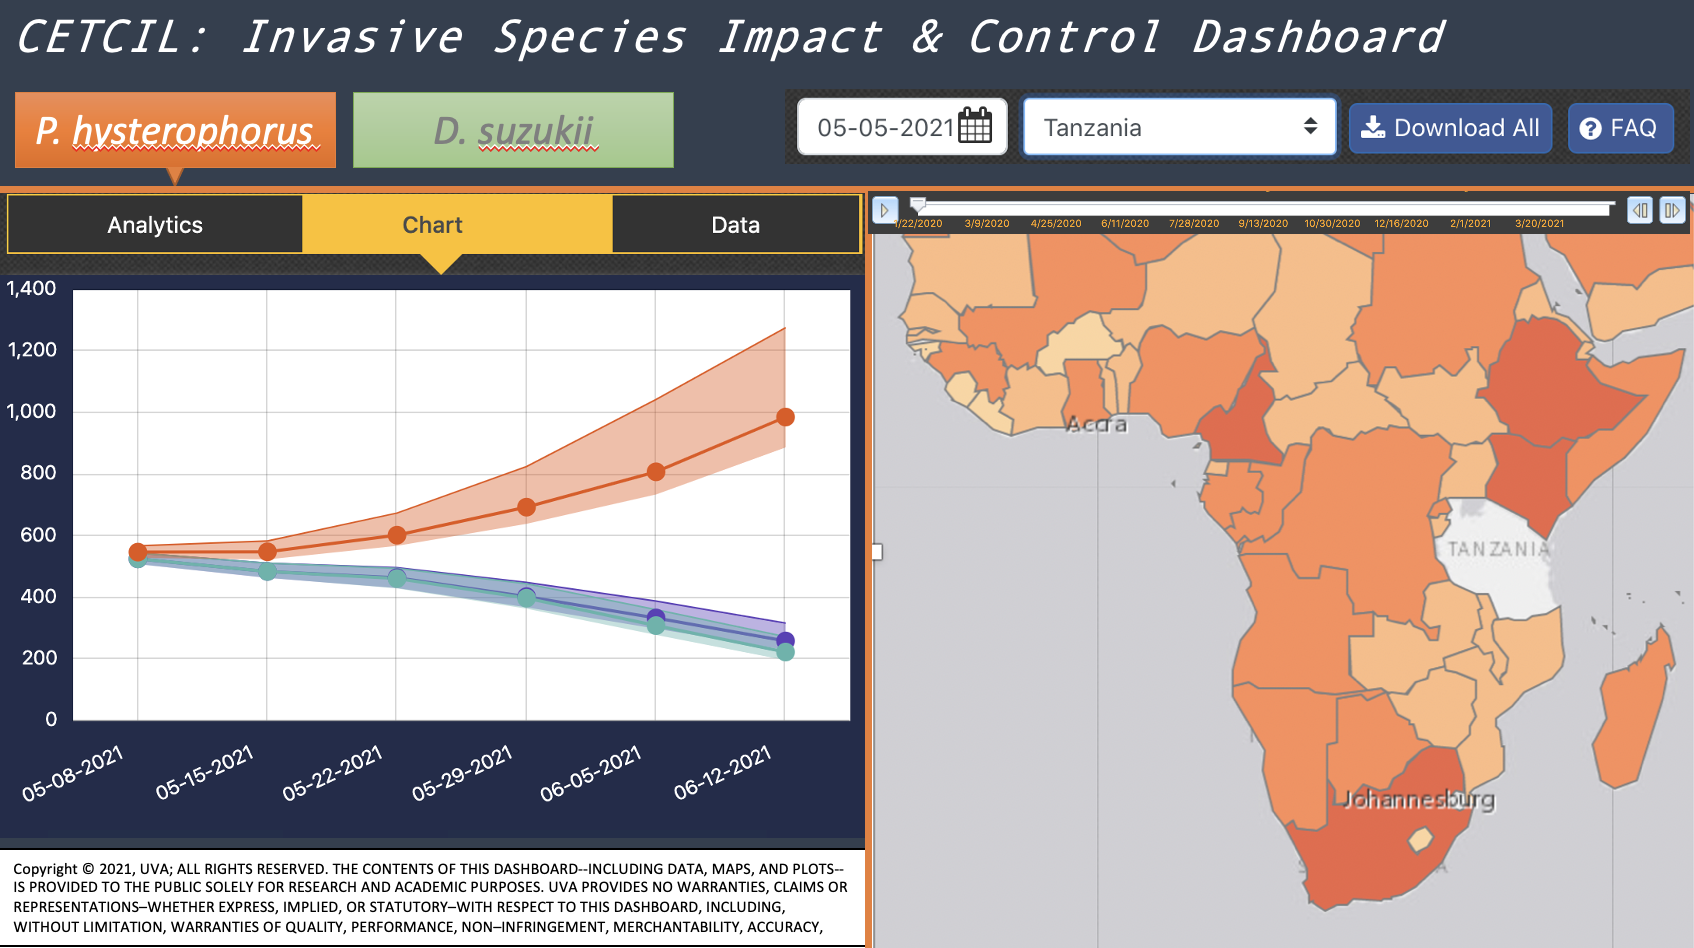
\includegraphics[width=8cm]{dashboard.png}};
\node [font=\bfseries,align=center,text width=8cm,shift={(0,.2)}] at (dash.north) {Decision Support System};
\node [below=of dash] (usaid) {
\includegraphics[width=5cm]{usaid.png}};
\node [font=\bfseries,below of=usaid] (ddl) {Development Data Library};

\draw[dedge,-*] (eco) -- ($(eeco)+(1,.4)$);
\draw (data) edge[edge,->] (eco);
\draw (data) edge[edge,->,out=70,in=180] (rs);
\draw (data) edge[edge,->,out=-70,in=180] (pa);
\draw (rs) edge[edge,->,out=0,in=140,looseness=1.25] (int);
\draw (pa) edge[edge,->,out=0,in=-140,looseness=1.25] (mon);
\draw (eco) edge[edge,->,out=10,in=210,looseness=1.25] (int);
\draw (eco) edge[edge,->,out=-10,in=-210,looseness=1.25] (mon);
\draw ($(dash.south)+(-2.8,0)$)
edge[edge,->,out=-120,in=-80,looseness=1.25] node [black!70,shift={(0,.6)}]
{Data inputs} (data);
\draw ($(dash.north)+(-2.8,0)$)
edge[edge,->,out=115,in=80,looseness=1.25] node [black!70,shift={(0,.9)}]
{Model inputs} (8,4);
\draw[->] (dash) edge[edge] ($(usaid)+(0,.3)$);

\begin{scope}[shift={(13,0)}]
    \fill[black!20] (0,0) -- ++(-.7,5) -- ++(-.2,0) -- ++(0,-10) -- ++(.2,0) -- cycle;
\end{scope}

\end{tikzpicture}
\end{document}




\draw (ana) edge[edge,->,out=0,in=180] (hyp);
\draw (hyp) edge[edge,->,out=-90,in=90] (sim);
\draw (sim) edge[edge,->,out=-180,in=0] (sana);
\draw (sana) edge[edge,->,out=-180,in=-40] (data);
\draw (ana) edge[edge,->,out=-70,in=170] node [explain,text width=2cm]
{Machine learned components of {\bf unknown processes}} (sim);

\end{tikzpicture}
\end{document}

